% ============================================ %

\documentclass[14pt,a4paper]{extarticle}

\usepackage[utf8]{inputenc}
\usepackage[ukrainian]{babel}
\usepackage{dsfont}
\usepackage[export]{adjustbox}
\usepackage[active]{srcltx}
\usepackage[final]{pdfpages}
\usepackage[hidelinks]{hyperref}

\usepackage{indentfirst}

\usepackage{verbatim}
\usepackage{amssymb}
\usepackage{physics}
\usepackage{amsmath}
\usepackage{algpseudocode}
\usepackage{algorithm}
\floatname{algorithm}{Algorithm}
\renewcommand{\algorithmicrequire}{\textbf{Input: }}
\renewcommand{\algorithmicensure}{\textbf{Output: }}
\newcommand{\algorithmreturn}{\textbf{return }}

% ============================================ %

\pagestyle{headings}    %нумерацiя сторiнок вгорi зправа i т.д.
\righthyphenmin=2                     %перенос 2 останніх букв
\pagenumbering{arabic}
\tolerance=400
\mathsurround=2pt
\hfuzz=1.5pt

% ============================================ %

\hoffset=-0.5cm            %+2.5cm -- вiдступ вiд лiвого краю
\voffset=-1.5cm             %+2.5cm -- вiдступ зверху
\oddsidemargin=0.1cm  %ліве поле
\topmargin=0.1cm         %верхнє поле
\headheight=0.5cm       %висота верхнього колонтитулу
\footskip=1cm               %висота нижнього колонтитулу
\headsep=0.3cm            %відступ від колонт. до тексту
\textwidth=17cm            %ширина сторінки
\textheight=25.5cm      %висота сторінки

% ============================================ %

% custom commands

\newcounter{e}
\setcounter{e}{0}
\newcommand{\n}{\refstepcounter{e} (\arabic{e})}

\newcounter{pic}
\setcounter{pic}{0}
\newcommand{\pic}[1]{\refstepcounter{pic} \vspace{-0.3cm}\textit{Рисунок \arabic{pic}\label{#1}.}}

\newcounter{tabl}
\setcounter{tabl}{0}
\newcommand{\tabl}[1]{\refstepcounter{tabl} \vspace{-0.3cm}\textit{Таблиця \arabic{tabl}\label{#1}.}}

\newcounter{dod}
\setcounter{dod}{0}
\newcommand{\dod}[1]{\refstepcounter{dod} \textit{Додаток \arabic{dod}\label{#1}.}}

\newtheorem{theorem}{Теорема}[section]
\newtheorem{defn}[theorem]{Означення}
\newtheorem{lemma}[theorem]{Лема}

\newcommand{\proof}{\textit{Доведення. \space}}
\numberwithin{equation}{section}
\numberwithin{figure}{section}

\newcommand{\tran}{^{T}}
\newcommand{\ith}{^{(i)}}
\newcommand{\lth}{^{(l)}}

\newcommand{\tabboxl}[2]{\parbox{#1}{\vspace{0.1cm} #2 \vspace{0.1cm} }}

\newcommand{\tabboxr}[2]{\parbox{#1}{\vspace{-0.3cm}
		\begin{flushright} #2 \end{flushright} \vspace{-0.3cm} }}

\newcommand{\tabboxc}[2]{\parbox{#1}{\vspace{-0.3cm}
		\begin{center} #2 \end{center} \vspace{-0.3cm} }}

% ============================================ %

% bibliography

\usepackage[
	backend=biber,
	style=numeric,
]{biblatex}

\nocite{statistical2013}
\nocite{elements2009}
\nocite{data2011}
\nocite{difference2019}
\addbibresource{literature.bib}

% ============================================ %

\begin{document}
	% ============================================ %
	\thispagestyle{empty}
	\begin{center}
		{\textbf{ЛЬВІВСЬКИЙ НАЦІОНАЛЬНИЙ УНІВЕРСИТЕТ \\ ІМЕНІ ІВАНА ФРАНКА}}\par
		{Факультет прикладної математики та інформатики \\ Кафедра обчислювальної математики}\par
		\vspace{40mm}
		{\textbf{\huge{Курсова робота}}}\par
		\vspace{5mm}
		{\large{Порівняння лінійних та нелінійних методів статистичного навчання для задачі з Kaggle}}\par
		\vspace{5mm}\par %subtitle
	\end{center}
	
	\vfill
	\vskip80pt
	
	\begin{flushleft}
		\hskip 8cm 
		Виконав студент III курсу групи
		\\ \hskip8cm
		ПМп-31 напрямку підготовки 
		\\ \hskip8cm
		(спеціальності)
		\\ \hskip8cm
		113 -- "Прикладна математика"
		\\ \hskip8cm
		Середович В.B.
	\end{flushleft}
	\begin{flushleft}
		\hskip8cm 
		Керівник: Вавричук В.Г.
	\end{flushleft}
	
	\vfill
	
	\begin{center}
		\large
		Львів - 2022
	\end{center}
	
	% ============================================ %
	% Зміст
	\newpage
	\thispagestyle{empty}
	%\addtocontents{toc}{\protect\thispagestyle{empty}}
	\tableofcontents
	
	% ============================================ %
	% Вступ	
	\newpage
	\thispagestyle{empty}
	\addcontentsline{toc}{section}{Вступ}
	\section*{Вступ}
	\begin{center}\end{center}
	Сучасний світ демонструє надшвидку динаміку змін, глобалізованість світу та доступність величезної кількості інформаційних ресурсів. Нові можливості підштовхують розвиток оцінки даних якомога глибше. Сфера статистики — це наука про навчання на даних. Статистичні знання допомагають використовувати правильні методи для збору даних, правильного аналізу та ефективного представлення результатів. Будь-якому спеціалісту в ході практичної діяльності доводиться здійснювати операції над кількісними даними, що здійснюються відповідно до математичних законів. Математична теорія змінюється порівняно повільно, проте технологія застосування математичних методів зазнала більш істотних змін. Активне впровадження безперешкодних комунікацій, якісної трансформації у безлічі галузей економіки та цифровізація суспільства у сфери здобутків штучного інтелекту та машинного навчання – лише частина трендів. Прогнозування дозволяє підприємствам ставити розумні та вимірювані цілі на основі поточних та історичних даних. Наявність точних даних і статистичних даних для аналізу допомагає підприємствам вирішувати, які зміни, зростання або покращення будуть визначені як успіх. В межах цієї роботи ми розглянемо деякі існуючі методи на основі алгоритмів, проаналізуємо їх та порівняємо їх між собою.	
	% ============================================ %
	
	\newpage
	\thispagestyle{empty}
	\section{Постановка задачі}	
	\begin{center}\end{center}
	
	Метою даної роботи є дослідження лінійних та нелінійних методів статистичного навчання та їх порівняння. В рамках роботи ми візьмемо набір даних про пацієнтів. Якщо ми визначимо, що існує зв’язок між хворобою серця та віком, холестерином, рівнем цукру, пульс та іншими параметрами, тоді ми можемо заздалегідь передбачити загрозу хвороби пацієнтів, тим самим рятувати життя. Іншими словами, наша мета — розробити точну модель, яку можна використовувати щоб спрогнозувати хворобу на основі параметрів людини. Ми будемо перевіряти методи навчання, використовувати їх для передбачення серцевої недостатності, оцінювати та порівнювати їх.

	\section{Порівняння машинного та статистичного навчання}
		
	Існують відмінності через історичні та соціологічні причини. Статистика є старшою галуззю ніж машинне навчання. Таким чином, ідеї щодо збору та аналізу даних у статистиці корінням сягають ще до того, як існували комп’ютери. Звичайно, ця галузь адаптувалася і з часом підходи до проблем і вибір теми дослідження в машинному та статистичному навчанні часто відрізняються між собою. \newline
	
	\textbf{Машинне навчання} — це область досліджень, присвячена розумінню та створенню методів, які «навчаються», тобто методів, які використовують дані для підвищення продуктивності певного набору завдань. \newline

    \textbf{Модель машинного навчання} називається алгоритм, який навчений розпізнавати певні типи закономірностей у даних. Модель навчають на основі набору інформації, надаючи їй алгоритм, який вона може використовувати для аналізу та навчання. \newline
    
    \textbf{Cтатистичне навчання} є однією з класичних структур для штучного інтелекту та області машинного навчання. Це набір математичних інструментів для вивчення функцій даних. Статистичне навчання базується на статистиці та функціональному аналізі. \newline
    
    \textbf{Статистична модель} — це модель даних, використовується для того, щоб зробити висновок про взаємозв'язки всередині них або щоб створити модель здатну передбачати майбутні значення. \newline
    
    Обидві галузі об'єднує одне питання: \textbf{як модель вчиться на даних?} \newline З роботи \cite{difference2019} можемо схарактеризувати машинне та статистичне навчання: \newline
	
	\textbf{Отже, машинне навчання:}
    
    \begin{itemize}
        \item навчається на даних без явно запрограмованих інструкцій
        \item може базуватись на основі мільярдів спостережень та атрибутів
        \item не залежить від припущень і в більшості випадків їх ігнорує
        \item визначає шаблони з набору даних за допомогою ітерацій, які вимагають набагато менше людських зусиль
    \end{itemize}
    
    \textbf{Натомість, статистичне навчання:}
    
    \begin{itemize}
        \item базується на меншому наборі даних з кількома атрибутами
        \item наголошує на передбаченнях, навчанні з наглядом, навчанні без нагляду та навчанні з частковим наглядом
        \item спирається на інтенсивну математику, яка базується на оцінювачі коефіцієнтів і вимагає хорошого розуміння даних
    \end{itemize}

    Загалом, ці дві сфери все більше змішуються між собою та обидві використовуються для розпізнавання образів, виявлення знань і аналізу даних.

    \newpage
    \thispagestyle{empty}
    \section{Оцінка функції $f$}
    
    Для оцінки даних ми будемо мати вхідні та вихідні параметри. Вхідні змінні зазвичай позначаються за допомогою символу $X$. Вхідні параметри мають такі назви як предиктори, незалежні змінні, ознаки або просто змінні. Вихідна змінна часто називається залежною змінною і зазвичай позначається символом $Y$. \newline
    
    Загалом, припустимо, що ми спостерігаємо вихідний параметр $Y$ та $p$ різних предикторів, $X_{1}, X_{2}, \ldots, X_{p}$. Ми припускаємо, що між $Y$ та $X=\left(X_{1}, X_{2}, \ldots, X_{p}\right)$ є певний зв’язок, який можна записати в загальному вигляді
    
    $$
    Y=f(X)+\epsilon
    $$
    
    Тут $f$ є деякою фіксованою, але невідомою функцією від $X_{1}, \ldots, X_{p}$, та $\epsilon$ випадкова похибка, незалежна від $X$ середнє значення дорівнює нулю. $f$ представляє систематичну інформацію, як $X$ описує $Y$. \newline
    
    По суті, \textbf{статистичне навчання} належить до набору підходів для оцінки $f$. \newline
    
    Є два основні критерії, за якими ми оцінюємо, точність $f$: \textbf{передбачення(prediction)} та \textbf{завдання висновку(Inference)}. \newline
	
	\textbf{Передбачення:} \newline
    
    У багатьох ситуаціях набір параметрів $X$ є доступний, але $Y$ непросто отримати. В цьому випадку, якщо випадкова похибка в середньому наближена до нуля, можемо прогнозувати $Y$ використовуючи
    $$
    \hat{Y}=\hat{f}(X)
    $$
    де $\hat{f}$ представляє нашу оцінку для $f$, і $\hat{Y}$ представляє результуючу оцінку $Y$. В цьому випадку, $\hat{f}$ трактують як чорна скринька (black box), маючи на увазі, що зазвичай вона не зацікавлена в точній формі $\hat{f}$, за умови, що вона дає точні прогнози для $Y$. \newline
    
    Припустимо, що $X_{1}, \ldots, X_{p}$ – це характеристики зразка крові пацієнта, які можна легко виміряти в лабораторії, а $Y$ – це змінна, що кодує ризик тяжкого захворювання пацієнта, побічна реакція на певний препарат. Природно намагатись спрогнозувати $Y$ за допомогою $X$, оскільки це може допомогти уникнути надання відповідного препарату пацієнтам, які мають високий ризик побічної реакції, тобто тим, для яких оцінка $Y$ є висока. \newline
    
    Точність $\hat{Y}$ як передбачення для $Y$ залежить від двох величин, які ми будемо називати зменшуваною (reducible) похибкою та не зменшуваною (irreducible) похибкою. Загалом, $\hat{f}$ не буде ідеальною оцінкою для $f$, і ця неточність призведе до певної похибки. Цю похибку можна зменшити, оскільки ми потенційно можемо підвищити точність $\hat{f}$, використовуючи для оцінки $f$ найбільш вдалу методику статистичного навчання. Однак, навіть якби можна було сформувати ідеальну оцінку для $f$, щоб наша оцінена відповідь мала вигляд $\hat{Y}=f(X)$, отримане передбачення все одно мало б певну похибку. Це відбувається тому, що $Y$ також є функцією $\epsilon$, яку, за визначенням, не можна передбачити за допомогою $X$. Тому мінливість, пов’язана з $\epsilon$, також впливає на точність наших прогнозів. Це поняття відоме як не зменшувана похибка, тому що, незалежно від того, наскільки добре ми оцінюємо $f$, ми не можемо зменшити похибку, яку вносить $\epsilon$. \newline
	
	Не зменшувана похибка є завжди більшою за нуль, тому що величина $\epsilon$ може містити невиміряні змінні, корисні для передбачення $Y$, а отже, $f$ не може використовувати їх для свого передбачення. Величина $\epsilon$ також може містити невиміряні варіації. Наприклад, ризик побічної реакції може змінюватися для деякого пацієнта в певний день, залежно від зміни самого препарату або загального самопочуття пацієнта в цей день. \newline
    
    Розглянемо задану оцінку $\hat{f}$ і набір предикторів $X$, що дає прогноз $\hat{Y}=\hat{f}(X)$. Припустимо, що і $\hat{f}$, і $X$ фіксовані.
    Тоді легко показати, що
    
    $$
    \begin{aligned}
        E(Y-\hat{Y})^{2} &=E[f(X)+\epsilon-\hat{f}(X)]^{2} \\
        &=\underbrace{[f(X)-\hat{f}(X)]^{2}}_{\text {Reducible }}+\underbrace{\operatorname{Var}(\epsilon)}_{\text {Irreducible }}
    \end{aligned}
    $$
    
    де $E(Y-\hat{Y})^{2}$ являє собою середнє квадратичну різницю між прогнозованим і фактичним значенням $Y$ і $\operatorname{Var}(\epsilon)$ та представляє дисперсію, пов'язану з випадкової похибки $\epsilon$. \newline
    
    \textbf{Завдання висновку}. \newline
    
    Зазвичай, нас цікавить розуміння того як зміна $Y$ впливає на $X_{1} \ldots, X_{p}$. У цій ситуації ми хочемо оцінити $f$, але наша мета не обов'язково полягає в тому, щоб робити прогнози для $Y$. Натомість ми хочемо зрозуміти зв’язок між $X$ та $Y$ або як змінюється $Y$ як функція від $X_{1}, \ldots, X_{p}$. Тепер $\hat{f}$ не можна розглядати як чорну скриньку, тому що нам потрібно знати його точну форму. У цьому контексті нас може цікавити відповідь на такі запитання:
    \begin{itemize}
        \item Які предиктори пов’язані з відповіддю? Часто буває, що лише невелика частина доступних предикторів істотно пов’язана з $Y$. Визначення кількох важливих предикторів серед великого набору можливих змінних може бути надзвичайно корисним, залежно від застосування.
        \item Який зв’язок між відповіддю та кожним окремим предиктором? Деякі предиктори можуть мати позитивний зв’язок з Y,  у сенсі
        що збільшення предиктора пов'язане зі збільшенням значень $Y$. Інші предиктори можуть мати протилежний вплив. Залежно від складності $f$, зв'язок між відповіддю та певним предиктором може також залежати від значень інших предикторів.
        \item Чи можна адекватно підсумувати зв’язок між $Y$ і кожним предиктором за допомогою лінійного рівняння, чи зв’язок є нелінійним? Історично, більшість методів оцінки $f$ мали лінійну форму. У деяких ситуаціях таке припущення є розумним або навіть бажаним. Але часто справжнє відношення є складнішим, і в цьому випадку лінійна модель не може забезпечити точне представлення зв’язку між вхідними та вихідними змінними.
    \end{itemize} 
    
    \newpage
    \thispagestyle{empty}
    \section{Категоризація методів навчання}
    
    \subsection{Задачі регресії та задачі класифікації}

    З підручника з основам статичтичного аналізу \cite{data2011} можемо схарактеризувати завдання апроксимації як завдання згладжування експериментальних даних. \textbf{Апроксимацією} називається процес підбору емпіричної формули $f(х)$ для встановленої з досвіду функціональної залежності
    $Y = f(x)$. Формула використовується для аналітичного представлення досліджуваних даних. Тобто завдання алгоритму моделювання полягає в тому, щоб знайти найкращу можливу функцію відображення з огляду на наявний час і ресурси. 

    Змінні можна поділити як \textbf{кількісні} або \textbf{якісні} (категоричні). Кількісні змінні набувають числових значень (вік людини, зріст чи дохід, вартість будинку). Якісні змінні набувають значення в одному з $K$ різних класів або категорій (чоловічий чи жіночий, марка A, B або C, так чи ні). 
    Зазвичай, до проблем з кількісною відповіддю, звертаються як до проблем \textbf{регресії}. Натомість задачі з якісною відповіддю часто називають проблемами \textbf{класифікації}. \newline
    
    \subsection{Лінійні та нелінійні методи}

    Лінійні та нелінійні підходи до оцінки $f$ мають певні характеристики. Припустимо, що існує набір з $n$ різних даних. Дані, які ми будемо використовувати для спостереження та тренування методів навчання, будемо називати навчальними даними. \newline
    
    \textbf{Модель регресії є лінійною}, коли доданками рівняння є константа та один або декілька параметрів помножених на незалежну зміну. Отже, тип рівняння регресії є лінійним за параметрами.
    $$
     Y = \beta_{0} + \beta_{1}X_{1} + \beta_{2}X_{2} + \dots + \beta_{k}X_{k} 
    $$
    
    Для \textbf{нелінійної регресії} дані спостереження моделюються функцією, яка є нелінійною комбінацією параметрів моделі та залежить від однієї або кількох незалежних змінних. Дані підбираються методом послідовних наближень. Тобто такий тип регресії використовується для моделювання зв'язку між незалежними змінними та залежними змінними. \newline
	\begin{figure}[h]
        \centering
        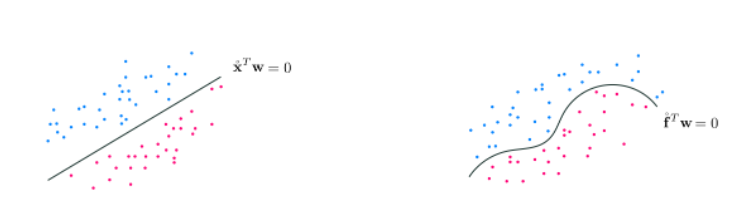
\includegraphics[width=0.9 \textwidth]{images/7.png}
        \caption{Ліворуч проілюстрована лінійна двокласна класифікація. Тут розділювальна межа визначається як $x^T w=0$ . Праворуч нелінійна двокласова класифікація досягається шляхом введення нелінійних перетворень ознак у нашу модель.}
        \label{fig:7}
    \end{figure}
    
    \textbf{Лінійна класифікація} належить до класифікації набору точок даних до дискретного класу на основі лінійної комбінації його змінних. Прикладом є логістична регресія. Лінійні методи класифікації використовуються коли навчальні дані не мають складних зв'язків та можуть бути лінійно розділені. \newline
    
    \textbf{Нелінійну класифікацію} використовують для розпізнавання екземплярів, коли навчальні дані мають складніші, нелінійні зв'язки та не можуть бути точно передбачені лінійними методами. 
    $$
    model(x, \theta) = w_{0} + f_{1}(x)w_{1} + f_{2}(x)w_{2} + \dots + f_{k}(x)w_{k}
    $$  
    $f_{1},f_{2},\dots,f_{k}$ є нелінійними параметризованими або не параметризованими функціями та $w_{0}-w_{k}$ представлені в наборі ваг $\theta$.
    
    \subsection{Параметричні та непараметричні методи}
    
    Загалом, більшість статистичних методів навчання для цього завдання можна схарактеризувати як \textbf{параметричні} або \textbf{непараметричні}. \newline

	Основна ідея \textbf{параметричного методу} полягає в тому, що існує набір фіксованих параметрів, які використовуються для визначення ймовірнісної моделі. Для параметричних методів ми попередньо знаємо, що сукупність є нормальною, або якщо ні, то ми можемо легко наблизити її за допомогою нормального розподілу. \newline
	
	Спочатку ми робимо припущення щодо функціональної форми або форми $f$. Наприклад, одне дуже просте припущення полягає в тому, що $f$ є лінійним у $X$:
	\begin{equation}
		\label{eq:parametric_model}
		f(X)=\beta_{0}+\beta_{1} X_{1}+\beta_{2} X_{2}+\ldots+\beta_{p} X_{p} .
	\end{equation} \newline
	Після припущення нам потрібно лише оцінити $p+1$ коефіцієнти $\beta_{0}, \beta_{1}, \ldots, \beta_{p}$. Обравши модель, далі нам потрібна процедура яка використовує навчальні дані для $f$ i $t$. У випадку лінійної моделі \ref{eq:parametric_model} нам необхідно оцінити параметри $\beta_{0}, \beta_{1}, \ldots, \beta_{p}$. Тобто ми хочемо знайти значення цих параметрів такі, що
	$$
	Y \approx \beta_{0}+\beta_{1} X_{1}+\beta_{2} X_{2}+\ldots+\beta_{p} X_{p} .
	$$
	
	Описаний підхід зводить проблему оцінки $f$ до проблеми оцінки набору параметрів. Припущення параметричної форми для $f$ спрощує проблему оцінки $f$, оскільки, як правило, набагато легше оцінити набір параметрів, таких як $\beta_{0}, \beta_{1}, \ldots, \beta_{p}$ у лінійній моделі \ref{eq:parametric_model}, ніж $f$. \newline 
		
    \textbf{Непараметричні методи} не роблять явних припущень про функціональну форму $f$. Замість цього вони шукають оцінку $f$, яка наближається до значення точки даних, наскільки це можливо. Такі підходи можуть мати велику перевагу над параметричними: уникаючи припущення певної функціональної форми для $f$, вони мають потенціал, щоб точно підігнати ширший діапазон можливих форм для $f$.\newline
    
    Будь-який параметричний підхід несе за собою ризик, що функціональна форма використана для оцінки $f$, буде дуже відмінною від істинної $f$, і в цьому випадку отримана модель буде погано наближати дані. Натомість непараметричні підходи повністю уникають цієї небезпеки, оскільки, не роблять припущень про форму $f$. Але непараметричні підходи мають недолік: оскільки вони не зводять задачу оцінки $f$ до малої кількості параметрів, для того, щоб отримати точну оцінити $f$, необхідна велика кількість спостережень. \newline
    	
	\subsection{Навчання з наглядом та без нагляду}
    
    Для навчання під наглядом для кожного спостереження предиктора $x_{i}, i = 1...n$ існує відповідна відповідь $y_{i}$. Ми хочемо підібрати модель, яка пов’язує відповідь до предиктора, з метою точного прогнозування відповіді (prediction) або розуміння зв'язку між відповіддю та предиктором (inference). Багато класичних статистичних методів навчання, таких як лінійна регресія та логістична регресія працюють у контрольованій області навчання. Для класифікації, контрольована модель навчання передбачає наявність вчителя або керівника, який класифікує навчальні приклади за класами та використовує інформацію про членство в кожному навчальному екземплярі. \newline
    
    Навпаки, навчання без нагляду описує ситуацію, в якій для кожного спостереження $i = 1...n$ існує вектор вимірювань $x_{i}$, але без відповідного $y_{i}$. В такому випадку, неможливо підібрати модель лінійної або логістичної регресії, оскільки немає змінної відповіді для вимірювань, яку можна було б передбачити. У цьому контексті ми в певному сенсі працюємо наосліп. Ситуація називається неконтрольованою, тому що дозволяє моделі працювати самостійно, щоб виявляти закономірності та інформацію, які не були виявлені раніше. До неконтрольованих методів належать такі методи як k-найближчих сусідів та деякі нейроні мережі.
    
    \newpage
    \thispagestyle{empty}
    \section{Оцінка якості методів}
    
    Жоден метод не домінує над усіма іншими на будь-якому наборі даних. На певному наборі даних може добре працювати один конкретний метод, але якийсь інший метод може краще працювати на схожому, але іншому наборі даних. Тому, завжди важливо приймати рішення про те, який метод дає найкращі результати на основі кожного окремого датасету.

    \subsection{Середня квадратична похибка (MSE)}

	У випадку \textbf{регресії}, найбільш часто використовуваною оцінкою алгоритму є середня квадратична похибка (MSE), яка визначається у вигляді \ref{eq:mse-formula}.

    \begin{equation}
        \label{eq:mse-formula}
    M S E=\frac{1}{n} \sum_{i=1}^{n}\left(y_{i}-\hat{f}\left(x_{i}\right)\right)^{2}
    \end{equation}

    де $\hat{f}(x_{i})$ – прогноз, який $\hat{f}$ дає для i-го спостереження. MSE буде невеликим, якщо передбачені відповіді дуже близькі до істинних відповідей і, навпаки, великим, якщо для деяких спостережень передбачені та істині відповіді суттєво відрізняються. \newline
    
    MSE в \ref{eq:mse-formula} обчислюється з використанням тренувальних даних. Загалом, для нас важливіше не те як модель працює на тренувальних даних, а те яка точність дає модель під час застосування методу до тестових даних. \newline
    
    Припустимо, що ми підігнали наш статистичний метод навчання до тренувальних спостережень $\left\{\left(x_{1}, y_{1}\right),\left(x_{2}, y_{2}\right), \ldots,\left(x_{n}, y_{n}\right)\right\}$, і отримуємо оцінку $\hat{f}$. Потім, ми можемо обчислити $\hat{f}(x_{1}), \hat{f}(x_{2}), \ldots, \hat{f}(x_{n})$. Якщо вони близькі до значень $y_{1}, y_{2}, \ldots, y_{n}$, то оцінка MSE, задана \ref{eq:mse-formula}, буде мала. Проте нас насправді не цікавить, чи $\hat{f}(x_{i}) \approx y_{i}$. Натомість ми хочемо знати, чи $\hat{f}(x_{0})$ приблизно дорівнює  $y_{0}$, де $\left(x_{0}, y_{0}\right)$ — це раніше невідоме тестове спостереження, яке не використовувалося для навчання методу статистичного навчання. Таким чином, ми хочемо вибрати метод, який дає найнижчий тестовий MSE, а не найнижчий навчальний MSE. \newline
	Іншими словами, якби у нас була велика кількість тестових спостережень, ми могли б обчислити
    \begin{equation}
        \label{eq:mse-formula-decomposition}
        \operatorname{Ave}\left(\hat{f}\left(x_{0}\right)-y_{0}\right)^{2},
    \end{equation}
    Середньоквадратичну похибку передбачення для цих тестових спостережень $\left(x_{0}, y_{0}\right)$. \newline
    
    \subsection{Компроміс зсуву та дисперсії}
    
    З підручника The Elements of Statistical Learning \cite{elements2009} можемо сказати що MSE, для заданого значення $x_{0}$, завжди розкладається на суму трьох основних величин: дисперсії $\hat{f}\left(x_{0}\right)$, квадратичне зміщення $\hat{f}\left(x_{0}\right)$ та дисперсії випадкової похибки $\epsilon$.
    \begin{equation}
        E\left(y_{0}-\hat{f}\left(x_{0}\right)\right)^{2}=\operatorname{Var}\left(\hat{f}\left(x_{ 0}\right)\right)+\left[\operatorname{Bias}\left(\hat{f}\left(x_{0}\right)\right)\right]^{2}+\operatorname{Var }(\epsilon)
    \end{equation}
    Тут позначення $E\left(y_{0}-\hat{f}\left(x_{0}\right)\right)^{2}$ визначає очікуваний тестовий $M S E$ і відноситься до середнього тестового $M S E$, який ми отримали б, якби ми неодноразово оцінювали $f$, використовуючи велику кількість навчальних наборів і перевіряли кожен на $x_{0}$. Загальний очікуваний тестовий $M S E$ можна обчислити шляхом усереднення $E\left(y_{0}-\hat{f}\left(x_{0}\right)\right)^{2}$ за всіма можливими значеннями $x_ {0}$ у тестовому наборі. \newline
    
    З рівняння \ref{eq:mse-formula-decomposition} маємо, що для того, щоб мінімізувати очікувану похибку тесту, нам потрібно вибрати метод статистичного навчання, який одночасно забезпечує низьку дисперсію та низьке зміщення. \newline

    \begin{figure}[h]
        \centering
        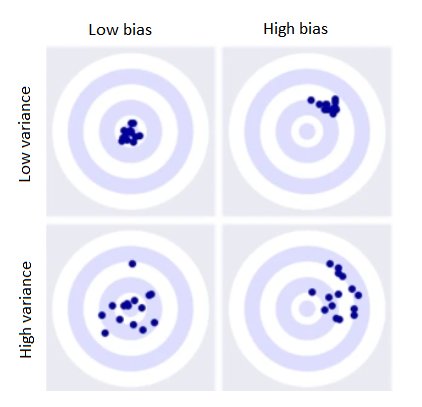
\includegraphics[width=0.6 \textwidth]{images/3.png}
        \caption{Пояснення дисперсії та зсуву на прикладі гри в дартс.}
        \label{fig:3}
    \end{figure}
    
    \textbf{Дисперсія} належить до величини, на яку змінилася б $\hat{f}$, якби ми оцінили її за допомогою іншого набору навчальних даних. Оскільки навчальні дані використовуються відповідно до статистичного методу навчання, різні набори навчальних даних призведуть до різних $\hat{f}$. Але в ідеалі оцінка $f$ не повинна сильно відрізнятися між навчальними наборами. Однак, якщо метод має високу дисперсію, то невеликі зміни в навчальних даних можуть призвести до великих змін у $\hat{f}$. Загалом, більш гнучкі статистичні методи мають більшу дисперсію та призводять до меншої упередженості.

    \subsection{Налаштування класифікації}

    Припустимо, що ми прагнемо оцінити $f$ на основі навчальних спостережень $\left\{\left(x_{1}, y_{1}\right), \ldots,\left(x_{n}, y_{n) }\right)\right\}$, де тепер $y_{1}, \ldots, y_{n}$ є якісними. Найпоширенішим підходом для кількісного визначення точності нашої оцінки $\hat{f}$ є \textbf{коефіцієнт помилок навчання}, які ми отримуємо при застосованні нашої оцінки $\hat{f}$ до навчальних спостережень:
    \begin{equation}
        \label{eq:accuracy_error}
    \frac{1}{n} \sum_{i=1}^{n} I\left(y_{i} \neq \hat{y}_{i}\right)
    \end{equation}
    Тут $\hat{y}_{i}$ – це передбачена мітка класу для $i$-го спостереження за допомогою $\hat{f}$, $I\left(y_{i} \neq \hat{y}_{i}\right)$ – це індикаторна змінна, яка дорівнює 1, якщо $y_{i} \neq \hat{y}_{i}$ і нуль, якщо $y_{i}=\hat{y}_{i}$. Якщо $I\left(y_{i} \neq \hat{y}_{i}\right)=0$, то $i$-е спостереження було класифіковано правильно за нашим методом класифікації, інакше його було неправильно класифіковано. Отже, рівняння \ref{eq:accuracy_error} обчислює частку неправильних класифікацій. \newline
 
	Рівняння \ref{eq:accuracy_error} називають коефіцієнтом помилок навчання, оскільки воно обчислюється на основі даних, які були використані для навчання нашого класифікатора. Рівень помилок тесту, пов'язаний з набором тестових спостережень у вигляді $\left(x_{0}, y_{0}\right)$, визначається як
    \begin{equation}
    \operatorname{Ave}\left(I\left(y_{0} \neq \hat{y}_{0}\right)\right)
    \end{equation}
    де $\hat{y}_{0}$ – це передбачена мітка класу, яка є результатом застосування класифікатора до тестового спостереження з предиктором $x_{0}$. Хорошим класифікатором є той, для якого тестова помилка \ref{eq:accuracy_error} найменша.
        
    \subsection{Перехресна перевірка (Cross validation)} 
    
    За відсутності дуже великого призначеного тестового набору, який можна використати, щоб оцінити частоту похибок тесту, можна використовувати ряд методик, щоб оцінити цю кількість, використовуючи наявні навчальні дані. Деякі методи роблять математичне корегування коефіцієнта похибок навчання, щоб оцінити частоту похибок тесту. \newline
    
    \textbf{Підхід набору перевірки} \newline
    
    Припустимо, що ми хотіли б оцінити похибку тесту, пов’язану з підгонкою конкретного статистичного методу навчання до набору спостережень.
    
	\begin{figure}[h]
		\centering
		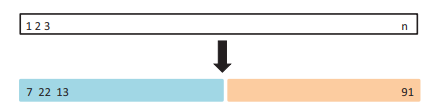
\includegraphics[width=0.9 \textwidth]{images/5.png}
		\caption{Схематичне відображення підходу до набору перевірки. Набір з $n$ спостережень випадковим чином розбивається на навчальний набір (синій колір) і набір перевірки (коричневий). Статистичний метод тренується на навчальному наборі, а його ефективність оцінюється на наборі перевірки.}
		\label{fig:5}
	\end{figure}

	Підхід включає випадковий поділ доступного набору спостереження на дві частини, навчальний набір і набір для перевірки. Модель тренується на навчальному наборі, а підібрана модель використовується для прогнозування відповіді на спостереженнях в наборі перевірки. На основі цієї перевірки, зазвичай рахується середньоквадратична похибка для оцінки точності отриманої моделі. \newline
	
	
	\textbf{Перехресна перевірка проблем класифікації} \newline
	
	Перехресна перевірка також може бути дуже корисним підходом у випадку класифікації, коли $Y$ є якісним. Тоді перехресна перевірка працює майже так само, за винятком того, що замість використання MSE для кількісної оцінки похибки тесту ми використовуємо кількість помилково класифікованих спостережень. Наприклад, у налаштуваннях класифікації частота помилок LOOCV приймає форму
	$$
		\mathrm{CV}_{(n)}=\frac{1}{n} \sum_{i=1}^{n} \operatorname{Err}_{i}
	$$
	де $\operatorname{Err}_{i}=I\left(y_{i} \neq \hat{y}_{i}\right)$. Коефіцієнт похибки у $k$-кратному $C V$ і частоти похибок набору визначаються аналогічним чином. \newline
	\subsection{Перехресна перевірка Leave One Out}
    В підручнику An Introduction to Statistical Learning \cite{statistical2013} представлено підхід до набору валідації LOOCV. Він передбачає поділ набору спостережень на дві частини. Однак замість створення двох підмножин порівнянного розміру, для набору перевірки використовується одне спостереження $\left(x_{1}, y_{1}\right)$, а решта спостережень $\left\{\left( x_{2}, y_{2}\right), \ldots,\left(x_{n}, y_{n}\right)\right\}$ складають навчальний набір. Метод статистичного навчання тренують на $n-1$ навчальних спостережень, а для виключеного спостереження робиться передбачення $\hat{y}_{1}$, використовуючи його значення $x_{1}$. Оскільки $\left(x_{1}, y_{1}\right)$ не використовувався в процесі підбору, MSE $_{1}=\left(y_{1}-\hat{y}_{1}\right)^{2}$ надає неупереджену оцінку помилки тесту. Але навіть попри те, що $\mathrm{MSE}_{1}$ є неупередженим для тестової помилки, це погана оцінка, оскільки вона дуже змінна, оскільки базується на одному спостереженні $\left(x_{1}, y_). {1}\right)$.
    
    Ми можемо повторити процедуру, вибравши $(x_{2}, y_{2})$ для даних перевірки, навчаючи статистичну модель на основі $n-1$ спостереженнях ${(x_{1}, y_{1}),(x_{3}, y_{3}), \ldots,(x_{n}, y_{n}) }$ і обчислення $\mathrm{MSE}_{2}=\left(y_{2}-\hat{y}_{2}\right)^{2}$. Повторення цього підходу $n$ разів створює $n$ квадратів похибок, $\operatorname{MSE}_{1}, \ldots$, MSE $_{n}$. Оцінка LOOCV для тестового MSE є середнім з цих $n$ оцінок похибок тесту:
    $$
    \mathrm{CV}_{(n)}=\frac{1}{n} \sum_{i=1}^{n} \operatorname{MSE}_{i}
    $$
        
    \begin{figure}[h!]
        \centering
        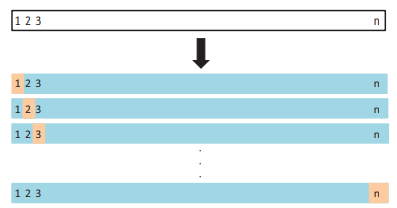
\includegraphics[width=0.6 \textwidth]{images/8.png}
        \caption{Набір з n точок даних багаторазово розбивається на навчальний набір (синій), що містить усі спостереження, крім одного, і набір перевірки, який містить лише це спостереження (коричневий). Тестова похибка оцінюється шляхом усереднення $n$ отриманих середньоквадратичних похибок. Перший тренувальний набір містить всі, крім спостереження 1, другий навчальний набір містить все, крім спостереження 2 і так далі...}
        \label{fig:8}
    \end{figure}

	\subsection{Перехресна перевірка K Fold}

    Перехресна перевірка K-Fold передбачає випадковий поділ множини спостережень на k груп, або згини, приблизно рівного розміру. Перший згин розглядається як набір перевірки, а метод тренують на решті $k-1$ згинів. Далі рахують середньоквадратичну похибку $MSE_{1}$ на основі спостережень у розгорнутому згині. Ця процедура повторюється k разів, кожного разу розглядається інша група спостережень як набір для перевірки. Цей процес призводить до $k$ оцінок похибки тесту, $MSE_{1}, MSE_{2}, \dots, MSE_{k}$. $K-$кратна оцінка CV обчислюється шляхом усереднення значень,
    $$
    CV(k) = \frac{1}{k} \sum_{i=1}^{k} MSE_{i}.
    $$

    \newpage
    \thispagestyle{empty}
    \section{Тренування і оцінка методів}
    
    \subsection{Оцінка датасету}
   Ми будемо використовувати датасет з ресурсу Kaggle, а саме дані про 918 пацієнтів з параметрами: (вік, стать, рівень холестерину, стенокардія, рівень цукру та пульс) вихідним параметром є хворе серце в людини чи ні. Датасет поділений на тренувальні та тестові в пропорції 80/20. 

	На гістограмі \ref{fig:age-distribution} зображено розподіл здорових та хворих пацієнтів по відношенню до віку. Як можна побачити, люди похилого віку частіше мають серцеві захворювання.
	
	\begin{figure}[h!]
		\centering
		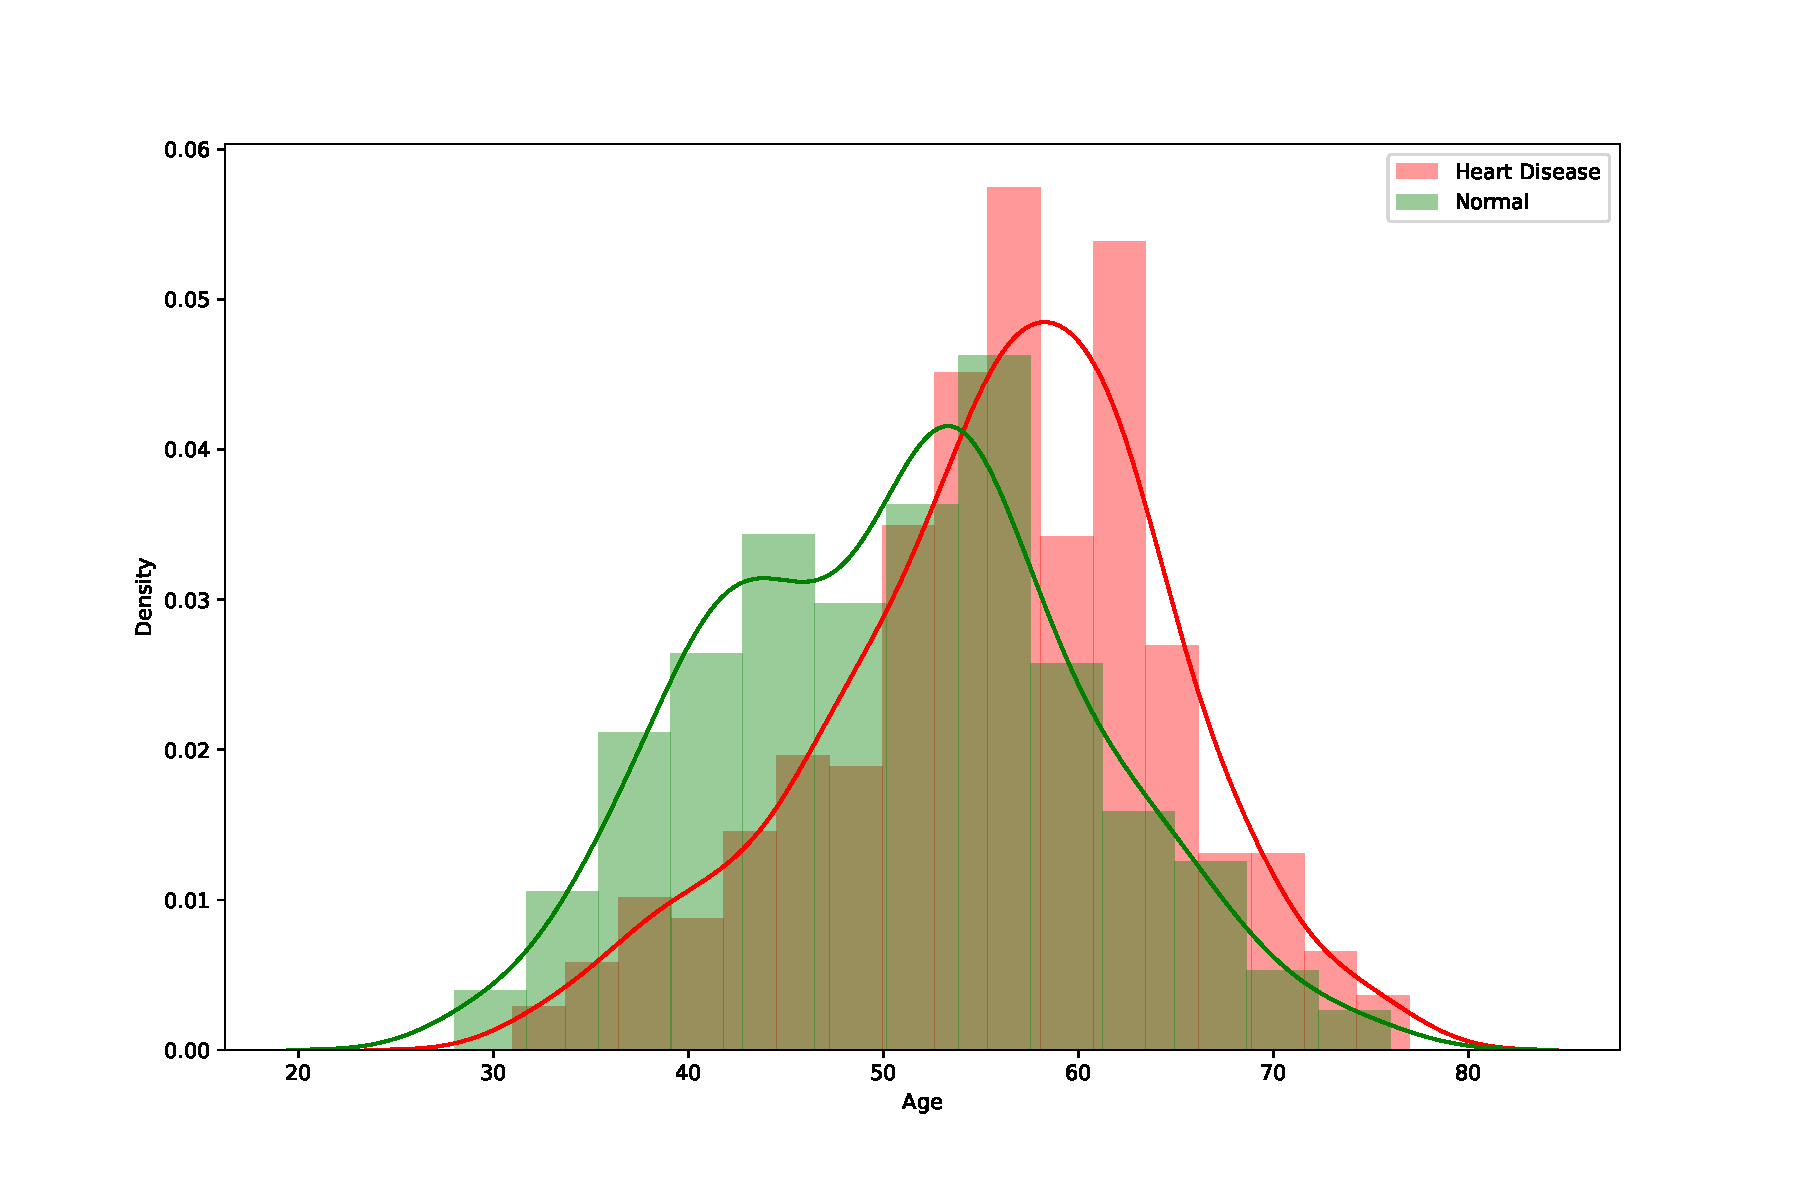
\includegraphics[width=1.1 \textwidth]{images/age_distribution.pdf}
		\caption{Гістограма віку хворих та здорових пацієнтів.}
		\label{fig:age-distribution}
	\end{figure}
	
	Відповідно до графіка кореляції між параметрами датасету \ref{fig:correlation} можна сказати, що існує позитивна кореляція серцевих захворювань людей з низькою максимальною частотою серцебиття та людей похилого віку.
	
	\begin{figure}[h!]
		\centering
		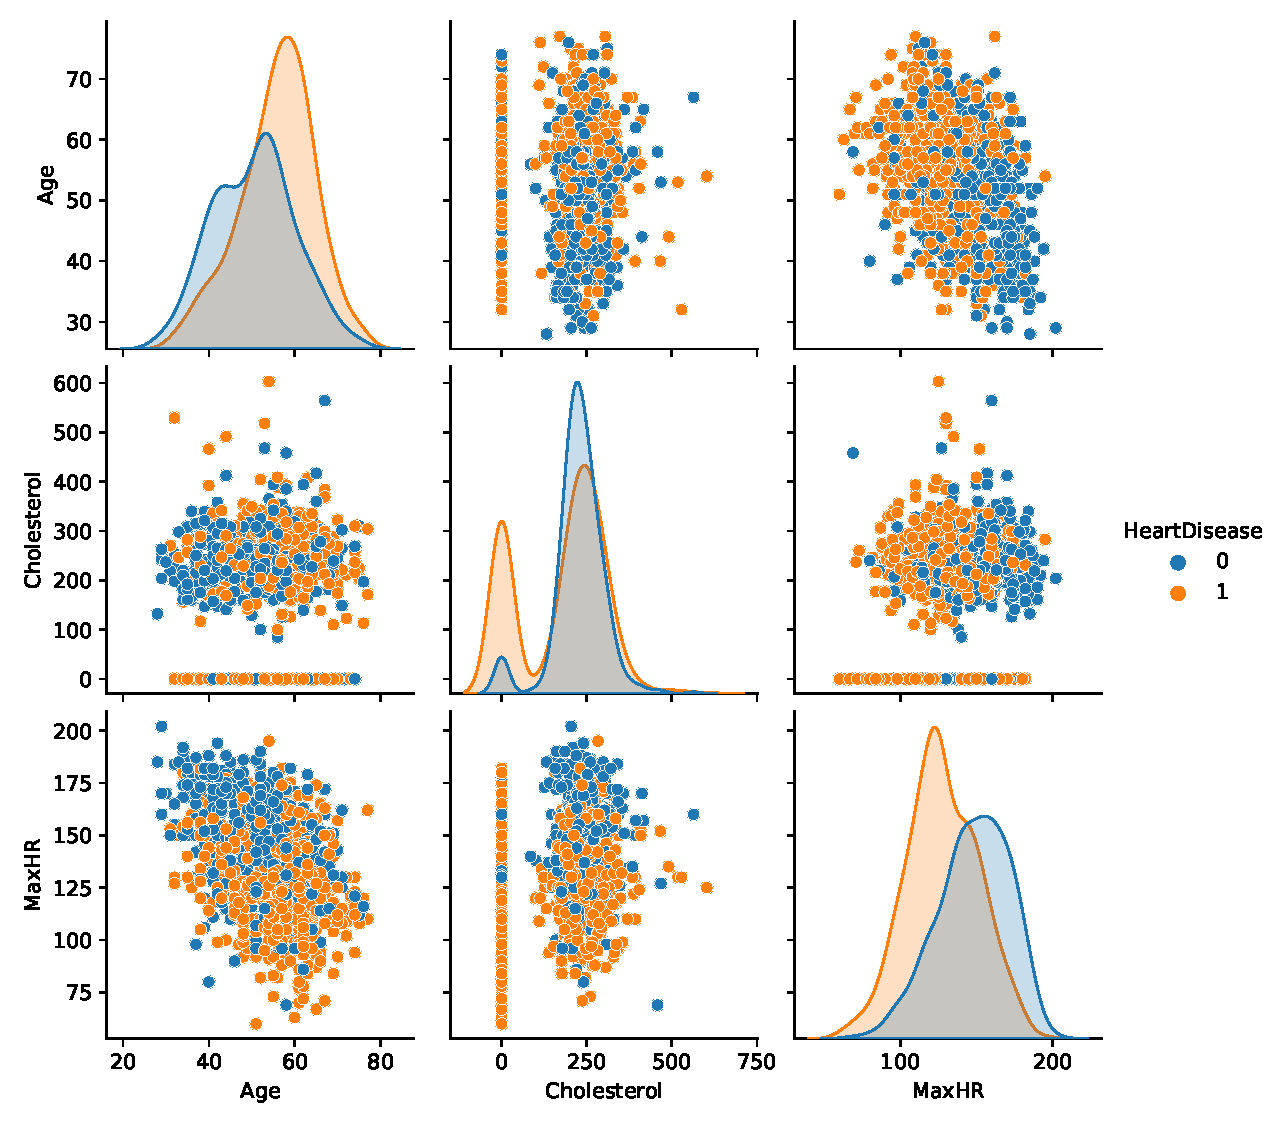
\includegraphics[width=1.1 \textwidth]{images/correlation.pdf}
		\caption{Графік кореляції між параметрами датасету.}
		\label{fig:correlation}
	\end{figure}
	
	Таким чином, на основі попередніх спостережень можна зробити висновок про те які параметри є більш важливі для побудови ефективної моделі виявлення серцевих захворювань.
	
	\subsection{Оцінка методів}
    
    Дана задача є задачею класифікації. Для порівняння методів були розглянуті лінійні методи класифікації, а саме: логістична регресія та лінійний дискримінантний аналіз.  
	Серед нелінійних методів були вибрані: метод k найближчих сусідів, квадратичний дискримінантний аналіз та нейронні мережі. Алгоритм логістичної регресії був реалізований самостійно коли інші алгоритми взяті з бібліотеки sklearn. \newline \newline \newline
        
    \begin{center} 
    	\begin{table}[!htbp] 
    		\centering 
    		\begin{tabular}{|c|c|c|c|c|} 
    			\hline \tabboxc{6cm}{Модель} 
    			& \tabboxc{2cm}{Точність} 
    			& \tabboxc{2cm}{MSE} 
    			& \tabboxc{2cm}{RMSE} 
    			& \tabboxc{2cm}{Time (seconds)} \\
    			\hline 
    			
    			\hline \tabboxc{6cm}{K найближчих сусідів} 
    			& \tabboxc{2cm}{72.28\%} 
    			& \tabboxc{2cm}{0.2771} 
    			& \tabboxc{2cm}{0.5264} 
    			& \tabboxc{2cm}{6.9e-7} \\
    			\hline 
    			
    			\hline \tabboxc{6cm}{Лінійний дискримінантний аналіз (LDA)} 
    			& \tabboxc{2cm}{84.78\%} 
    			& \tabboxc{2cm}{0.1521} 
    			& \tabboxc{2cm}{0.39}
    			& \tabboxc{2cm}{2.92e-3} \\
    			\hline 
    			
    			\hline \tabboxc{6cm}{Квадратичний дискримінантний аналіз (QDA)} 
    			& \tabboxc{2cm}{74.45\%} 
    			& \tabboxc{2cm}{0.2554} 
    			& \tabboxc{2cm}{0.5054}
    			& \tabboxc{2cm}{1.92e-3} \\
    			\hline 
    			
    			\hline \tabboxc{6cm}{Нейронні мережі} 
    			& \tabboxc{2cm}{83.69\%} 
    			& \tabboxc{2cm}{0.163} 
    			& \tabboxc{2cm}{0.4037}
    			& \tabboxc{2cm}{1.88} \\
    			\hline 
    			
    			\hline \tabboxc{6cm}{Логістична регресія} 
    			& \tabboxc{2cm}{82.60\%} 
    			& \tabboxc{2cm}{0.1739} 
    			& \tabboxc{2cm}{0.417}
    			& \tabboxc{2cm}{6,3e-2} \\
    			\hline 
    			    			
    		\end{tabular}  
    		\label{tab:model-hyperparameters} 
    		\caption{Оцінка передбачень моделі на тестовому наборі даних.}
    	\end{table} 
    \end{center}

    В таблиці \ref{tab:model-hyperparameters} ми спостерігаємо ефективність лінійних та нелінійних моделей. Найкращий результат за точністю показує лінійний дискримінантний аналіз. Інший лінійний метод, а саме логістична регресія також показує добрий результат. Гіршим себе проявляє K наближених сусідів. Також можемо помітити що лінійні алгоритми загалом працюють швидше за нелінійні.
    
    \begin{center} 
    	\begin{table}[!htbp] 
    		\centering 
    		\begin{tabular}{|c|c|c|} 
    			\hline \tabboxc{6cm}{Модель} 
    			& \tabboxc{4cm}{Leave One Out} 
    			& \tabboxc{4cm}{K-Fold} \\
    			\hline 
    			
    			\hline \tabboxc{6cm}{K найближчих сусідів} 
    			& \tabboxc{4cm}{76.6\%} 
    			& \tabboxc{4cm}{76.4\%} \\ 
    			\hline 
    			
    			\hline \tabboxc{6cm}{Лінійний дискримінантний аналіз (LDA)} 
    			& \tabboxc{4cm}{86.2\%} 
    			& \tabboxc{4cm}{85.8\%} \\ 
    			\hline 
    			
    			\hline \tabboxc{6cm}{Квадратичний дискримінантний аналіз (QDA)} 
    			& \tabboxc{4cm}{58.3\%} 
    			& \tabboxc{4cm}{68.8\%} \\ 
    			\hline 
    			
    			\hline \tabboxc{6cm}{Нейронні мережі} 
    			& \tabboxc{4cm}{84.6\%} 
    			& \tabboxc{4cm}{83.8\%} \\ 
    			\hline 
    			
    			\hline \tabboxc{6cm}{Логістична регресія} 
    			& \tabboxc{4cm}{85.7\%} 
    			& \tabboxc{4cm}{85.5\%} \\ 
    			\hline 
    			
    		\end{tabular}  
    		\label{tab:cross-validation} 
    		\caption{Таблиця оцінки моделей перехресної перевірки.}
    	\end{table} 
    \end{center}
    
    З таблиці перехресної перевірки \ref{tab:cross-validation} ми підтверджуємо наші спостереження щодо якості метода для нашої задачі. Лінійні методи проявляють себе краще.
    
    \newpage
    \thispagestyle{empty}
    \section{Висновок}
    
    В ході цієї роботи ми розглянули зв'язок між статистичним та машинним навчанням. Розглянули ідею оцінки функції, різні категорії на які розподіляються статистичні методи та способи оцінювати та порівняння їх між собою. \newline

	Для поставленої задачі необхідно було обрати датасет разом з ним лінійні та нелінійні методи статистичного навчання. Також ми використали методи оцінки для наших статистичних навчань такі як перехресні перевірки, коефіцієнт помилок навчання та середня квадратична похибка. \newline

	За результатами експериментів можна сказати що для даного конкретного дадасету лінійні методи проявили себе краще як за часом виконання, так і за точністю результатів. Також для простих датасетів з переважно лінійними зв'язками в даних доцільніше використовувати лінійні методи навчання, адже вони менш схильні до перетренування. \newline

	Підсумовуючи наведене можна стверджувати що і лінійні та нелінійні методи мають свої переваги та недоліки. Чим більш обмежувальний та негнучкий є метод, тим простіше зрозуміти зв'язок між предикторами та відповіддю та він буде краще інтерпретуватись. А більш гнучкі методи краще апроксимує, але є більш вибагливими за кількістю тренувальних даних та потребують більше часу на тренування. Вибір найкращого підходу може бути однією з найскладніших частин виконання статистичного навчання. Для того, щоб оцінити ефективність статистичного методу навчання нам потрібен спосіб виміряти, наскільки добре його передбачення  фактично відповідають спостережуваним даним.\newline

	\newpage
	\thispagestyle{empty}
	\printbibliography[title={Література}]
	
\end{document}